% 高斯光束

\begin{issues}
\issueDraft
\issueMissDepend
\issueOther{翻译成中文}
\end{issues}

Wave Eq.
\begin{equation}
\laplacian \bvec E - \frac{1}{c^2} \pdv[2]{\bvec E}{t} = 0
\end{equation}
assume propagation within small angle of $z$ axis
\begin{equation}
\bvec E = \uvec \epsilon E(\bvec r, t) = 2\uvec \epsilon U(x, y, z) \E^{\I (kz - \omega t)}
\end{equation}
$U(x, y, z)$ is the envelope. Plug in, use ‘slowly varying envelope approximation’
\begin{equation}
2\I k\pdv{U}{z} = \pdv[2]{U}{x} + \pdv[2]{U}{y}
\end{equation}
The general solution is a linear combination of the following basis
\begin{equation}
U_{mn}(x, y, z) = \frac{C}{w(z)} \exp[-\frac{r^2}{w^2(z)}]\exp[\I k\frac{r^2}{2R(z)}] H_m\qty[\frac{\sqrt{2}x}{w(z)}] H_n \qty[\frac{\sqrt{2} y}{w(z)}] \E^{-\I \phi_{mn}(z)}
\end{equation}
\begin{equation}
\phi_{mn}(z) = (m+n+1)\tan^{-1}(z/z_R)
\end{equation}
\begin{equation}
w(z) = w_0\sqrt{1 + z^2/z_R^2}
\qquad
R(z) = z + z_R^2 / z
\qquad
z_R = \pi w_0^2 / \lambda
\end{equation}
\begin{equation}
H_0 = 1 \qquad H_1 = 2x \qquad H_2 = 4x^2 - 1
\end{equation}
This is called the \textbf{Hermite-Gauss mode}, denoted $TEM_{mn}$. $H$ are Hermite polynomials and $\phi$ is the \textbf{Gouy phase-shift}, $z_R$ is the \textbf{Rayleigh length}. The second exp factor makes the wave front a spherical wave with curvature $R(z)$, because
\begin{equation}
l - R = \sqrt{R^2 + z^2} - R \approx \frac{r^2}{2R}
\end{equation}

\begin{figure}[ht]
\centering
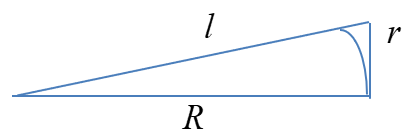
\includegraphics[width=5cm]{./figures/GausBm_1.png}
\caption{triangle} \label{GausBm_fig1}
\end{figure}

$TEM_{00}$ is the \textbf{fundamental Gaussian mode}.

In cylindrical coordinates, the basis change to \textbf{Laguerre-Gauss modes} $TEM_{lm}^*$
\begin{equation}
U_{lm}(r, \theta, z) = \frac{C'}{w(z)} \qty[\frac{\sqrt{2}r}{w(z)}]^{\abs{m}} \exp[-\frac{r^2}{w^2(z)}] \exp[\I \frac{r^2}{2R(z)}] L_l^{\abs{m}} \qty[\frac{2r^2}{w^2(z)}] \E^{\I m\theta} \E^{-\I \phi_{lm}(z)}
\end{equation}
\begin{equation}
\phi_{lm}(z) = (2l + \abs{m} + 1) \tan^{-1} (z/z_R)
\end{equation}
This is analogous to solving SHO in polar coordiantes while Hermite-Gauss modes are in Cartesian coordinates. 
